\documentclass{beamer}
\usepackage[outputdir=build]{minted}
\usepackage[skins,minted,breakable]{tcolorbox}
\usepackage[spanish]{babel}
\usepackage{subcaption}
\usetikzlibrary{matrix,backgrounds}
\usepackage{multirow}
\usepackage{multicol}
\usepackage{adjustbox}

\graphicspath{ {../img/} {../../LaTeX/img/} {/home/csp98/latex/img/}}
\selectlanguage{spanish}
\usepackage[utf8]{inputenc}
\usetheme{PaloAlto}
\setbeamerfont{section in sidebar}{size=\fontsize{2}{4}\selectfont}
\setbeamerfont{subsection in sidebar}{size=\fontsize{2}{3}\selectfont}
\setbeamerfont{subsubsection in sidebar}{size=\fontsize{2}{2}\selectfont}

\setbeamerfont{section in toc}{size=\footnotesize}
\setbeamerfont{subsection in toc}{size=\scriptsize}
\setbeamerfont{subsubsection in toc}{size=\tiny}

\usetikzlibrary{arrows,positioning,automata,shadows,fit,shapes,calc}



\title{Práctica 3}
\date{4 de mayo de 2018}
\subtitle{El viajante de comercio}

\author{María Jesús López Salmerón \\ Nazaret Román Guerrero \\ Laura Hernández Muñoz \\ José Baena Cobos  \\ Carlos Sánchez Páez}

\makeatletter
  \setbeamertemplate{sidebar \beamer@sidebarside}%{sidebar theme}
  {
    \beamer@tempdim=\beamer@sidebarwidth%
    \advance\beamer@tempdim by -6pt%
    \insertverticalnavigation{\beamer@sidebarwidth}%
    \vfill
    \ifx\beamer@sidebarside\beamer@lefttext%
    \else%
      \usebeamercolor{normal text}%
      \llap{\usebeamertemplate***{navigation symbols}\hskip0.1cm}%
      \vskip2pt%
    \fi%
}%
\makeatother

\subject{Algorítmica}
\AtBeginSection[]
  {
     \begin{frame}<beamer>
     \frametitle{Índice}
     \tableofcontents[currentsection]
     \end{frame}
  }
\AtBeginSubsection[]
{
  \begin{frame}<beamer>{Índice}
    \tableofcontents[currentsection,currentsubsection]
  \end{frame}
}

% Let's get started
\begin{document}
\centering
\begin{frame}
  \titlepage
\end{frame}

\begin{frame}{Índice}
  \tableofcontents
  % You might wish to add the option [pausesections]
\end{frame}

\section{Presentación del problema}


\begin{frame}[fragile]{El viajante de comercio}

\begin{tikzpicture}[-,>=latex,shorten >=1pt,auto,node distance=6cm, main node/.style={circle,draw},scale=0.4]
	\tikzstyle{every node}=[font=\tiny]
	\draw (3,19) node(a) [circle, draw,fill=red!45] {1}
          	 (-6,13) node(b) [circle, draw,fill=red!45] {2}
          	 (-2,5) node(c) [circle, draw,fill=red!45] {3}
          	 (12,13) node(d) [circle, draw,fill=red!45] {4}
          	 (8,5) node(e) [circle, draw,fill=red!45] {5};
	%\draw[draw=blue] (a) to (b);
	\path[draw,thick] (a) edge node {$c_1$} (b);
	\path[draw,thick] (a) edge node {$c_2$} (c);
	\path[draw,thick] (a) edge node {$c_3$} (d);
	\path[draw,thick] (a) edge node {$c_4$} (e);
	\path[draw,thick] (b) edge node {$c_5$} (c);
	\path[draw,thick] (b) edge node {$c_6$} (d);
	\path[draw,thick] (b) edge node {$c_7$} (e);
	\path[draw,thick] (c) edge node {$c_8$} (d);
	\path[draw,thick] (c) edge node {$c_9$} (e);
	\path[draw,thick] (d) edge node {$c_{10}$} (e);

\end{tikzpicture}

\end{frame}

\begin{frame}[fragile]{El viajante de comercio}

\begin{tikzpicture}[-,>=latex,shorten >=1pt,auto,node distance=6cm, main node/.style={circle,draw},scale=0.4]
	\tikzstyle{every node}=[font=\tiny]
	\draw (3,19) node(a) [circle, draw,fill=yellow!45] {1}
          	 (-6,13) node(b) [circle, draw,fill=red!45] {2}
          	 (-2,5) node(c) [circle, draw,fill=red!45] {3}
          	 (12,13) node(d) [circle, draw,fill=red!45] {4}
          	 (8,5) node(e) [circle, draw,fill=red!45] {5};
	%\draw[draw=blue] (a) to (b);
	\path[draw=blue,thick] (a) edge node {$c_1$} (b);
	\path[draw,thick] (a) edge node {$c_2$} (c);
	\path[draw=blue!40,thick] (a) edge node {$c_3$} (d);
	\path[draw,thick] (a) edge node {$c_4$} (e);
	\path[draw=blue,thick] (b) edge node {$c_5$} (c);
	\path[draw,thick] (b) edge node {$c_6$} (d);
	\path[draw,thick] (b) edge node {$c_7$} (e);
	\path[draw,thick] (c) edge node {$c_8$} (d);
	\path[draw=blue,thick] (c) edge node {$c_9$} (e);
	\path[draw=blue,thick] (d) edge node {$c_{10}$} (e);

\end{tikzpicture}

Una solución: $\{1,2,3,5,4,1\}$. Coste = $c_1+c_5+c_9+c_{10}+c_3$.
\end{frame}

\section{Heurísticas empleadas}

\subsection{Vecino más cercano}

\begin{frame}[fragile]{Vecino más cercano}

\begin{itemize}
	\item \textbf{Conjunto de candidatos}. Ciudades a visitar.
\end{itemize}

\end{frame}

\begin{frame}[fragile]{Vecino más cercano}

\begin{itemize}
	\item \textbf{Conjunto de candidatos}. Ciudades a visitar.
	\item \textbf{Conjunto de seleccionados}. Ciudades que vayamos incorporando al circuito.
\end{itemize}

\end{frame}

\begin{frame}[fragile]{Vecino más cercano}

\begin{itemize}
	\item \textbf{Conjunto de candidatos}. Ciudades a visitar.
	\item \textbf{Conjunto de seleccionados}. Ciudades que vayamos incorporando al circuito.
	\item \textbf{Función solución}. Todas las ciudades han sido visitadas y hemos vuelto a la primera.
\end{itemize}

\end{frame}

\begin{frame}[fragile]{Vecino más cercano}

\begin{itemize}
	\item \textbf{Conjunto de candidatos}. Ciudades a visitar.
	\item \textbf{Conjunto de seleccionados}. Ciudades que vayamos incorporando al circuito.
	\item \textbf{Función solución}. Todas las ciudades han sido visitadas y hemos vuelto a la primera.
	\item \textbf{Función de factibilidad}. La ciudad no ha sido visitada aún.
\end{itemize}

\end{frame}

\begin{frame}[fragile]{Vecino más cercano}

\begin{itemize}
	\item \textbf{Conjunto de candidatos}. Ciudades a visitar.
	\item \textbf{Conjunto de seleccionados}. Ciudades que vayamos incorporando al circuito.
	\item \textbf{Función solución}. Todas las ciudades han sido visitadas y hemos vuelto a la primera.
	\item \textbf{Función de factibilidad}. La ciudad no ha sido visitada aún.
	\item \textbf{Función de selección}. Aquella ciudad que sea más cercana a la ciudad en la que nos encontramos.
\end{itemize}

\end{frame}

\begin{frame}[fragile]{Vecino más cercano}

\begin{tikzpicture}[-,>=latex,shorten >=1pt,auto,node distance=6cm, main node/.style={circle,draw},scale=0.4]
	\tikzstyle{every node}=[font=\tiny]
	\draw (3,19) node(a) [circle, draw,fill=yellow!45] {1}
          	 (-6,13) node(b) [circle, draw,fill=red!45] {2}
          	 (-2,5) node(c) [circle, draw,fill=red!45] {3}
          	 (12,13) node(d) [circle, draw,fill=red!45] {4}
          	 (8,5) node(e) [circle, draw,fill=red!45] {5};
	%\draw[draw=blue] (a) to (b);
	\path[draw,thick] (a) edge node {$1$} (b);
	\path[draw,thick] (a) edge node {$2$} (c);
	\path[draw,thick] (a) edge node {$3$} (d);
	\path[draw,thick] (a) edge node {$4$} (e);
	\path[draw,thick] (b) edge node {$5$} (c);
	\path[draw,thick] (b) edge node {$6$} (d);
	\path[draw,thick] (b) edge node {$7$} (e);
	\path[draw,thick] (c) edge node {$8$} (d);
	\path[draw,thick] (c) edge node {$9$} (e);
	\path[draw,thick] (d) edge node {$10$} (e);

\end{tikzpicture}

Comenzamos en la ciudad 1.

\end{frame}

\begin{frame}[fragile]{Vecino más cercano}

\begin{tikzpicture}[-,>=latex,shorten >=1pt,auto,node distance=6cm, main node/.style={circle,draw},scale=0.4]
	\tikzstyle{every node}=[font=\tiny]
	\draw (3,19) node(a) [circle, draw,fill=yellow!45] {1}
          	 (-6,13) node(b) [circle, draw,fill=red!45] {2}
          	 (-2,5) node(c) [circle, draw,fill=red!45] {3}
          	 (12,13) node(d) [circle, draw,fill=red!45] {4}
          	 (8,5) node(e) [circle, draw,fill=red!45] {5};
	%\draw[draw=blue] (a) to (b);
	\path[draw=blue,thick] (a) edge node {$1$} (b);
	\path[draw,thick] (a) edge node {$2$} (c);
	\path[draw,thick] (a) edge node {$3$} (d);
	\path[draw,thick] (a) edge node {$4$} (e);
	\path[draw,thick] (b) edge node {$5$} (c);
	\path[draw,thick] (b) edge node {$6$} (d);
	\path[draw,thick] (b) edge node {$7$} (e);
	\path[draw,thick] (c) edge node {$8$} (d);
	\path[draw,thick] (c) edge node {$9$} (e);
	\path[draw,thick] (d) edge node {$10$} (e);

\end{tikzpicture}

Añadimos la más cercana: ciudad 2.

\end{frame}

\begin{frame}[fragile]{Vecino más cercano}

\begin{tikzpicture}[-,>=latex,shorten >=1pt,auto,node distance=6cm, main node/.style={circle,draw},scale=0.4]
	\tikzstyle{every node}=[font=\tiny]
	\draw (3,19) node(a) [circle, draw,fill=yellow!45] {1}
          	 (-6,13) node(b) [circle, draw,fill=red!45] {2}
          	 (-2,5) node(c) [circle, draw,fill=red!45] {3}
          	 (12,13) node(d) [circle, draw,fill=red!45] {4}
          	 (8,5) node(e) [circle, draw,fill=red!45] {5};
	%\draw[draw=blue] (a) to (b);
	\path[draw=blue,thick] (a) edge node {$1$} (b);
	\path[draw,thick] (a) edge node {$2$} (c);
	\path[draw,thick] (a) edge node {$3$} (d);
	\path[draw,thick] (a) edge node {$4$} (e);
	\path[draw=blue,thick] (b) edge node {$5$} (c);
	\path[draw,thick] (b) edge node {$6$} (d);
	\path[draw,thick] (b) edge node {$7$} (e);
	\path[draw,thick] (c) edge node {$8$} (d);
	\path[draw,thick] (c) edge node {$9$} (e);
	\path[draw,thick] (d) edge node {$10$} (e);

\end{tikzpicture}

Añadimos la más cercana: ciudad 3.

\end{frame}

\begin{frame}[fragile]{Vecino más cercano}

\begin{tikzpicture}[-,>=latex,shorten >=1pt,auto,node distance=6cm, main node/.style={circle,draw},scale=0.4]
	\tikzstyle{every node}=[font=\tiny]
	\draw (3,19) node(a) [circle, draw,fill=yellow!45] {1}
          	 (-6,13) node(b) [circle, draw,fill=red!45] {2}
          	 (-2,5) node(c) [circle, draw,fill=red!45] {3}
          	 (12,13) node(d) [circle, draw,fill=red!45] {4}
          	 (8,5) node(e) [circle, draw,fill=red!45] {5};
	%\draw[draw=blue] (a) to (b);
	\path[draw=blue,thick] (a) edge node {$1$} (b);
	\path[thick] (a) edge node {$2$} (c);
	\path[thick] (a) edge node {$3$} (d);
	\path[thick,draw=blue!40] (a) edge node {$4$} (e);
	\path[draw=blue,thick] (b) edge node {$5$} (c);
	\path[thick] (b) edge node {$6$} (d);
	\path[thick] (b) edge node {$7$} (e);
	\path[draw=blue,thick] (c) edge node {$8$} (d);
	\path[thick] (c) edge node {$9$} (e);
	\path[draw=blue,thick] (d) edge node {$10$} (e);

\end{tikzpicture}

Como último paso volvemos al inicio. Solución: $\{1,2,3,4,5,1\}$. Coste=28.
\end{frame}

\begin{frame}[fragile]{Vecino más cercano}
Para obtener soluciones más óptimas, probamos con todas las posibles ciudades de inicio.
\end{frame}

\subsection{Inserción más económica}

\begin{frame}[fragile]{Inserción más económica}

\begin{itemize}
	\item \textbf{Conjunto de candidatos}. Ciudades a visitar.
\end{itemize}

\end{frame}

\begin{frame}[fragile]{Inserción más económica}

\begin{itemize}
	\item \textbf{Conjunto de candidatos}. Ciudades a visitar.
	\item \textbf{Conjunto de seleccionados}. Ciudades que vayamos incorporando al circuito.
\end{itemize}

\end{frame}

\begin{frame}[fragile]{Inserción más económica}

\begin{itemize}
	\item \textbf{Conjunto de candidatos}. Ciudades a visitar.
	\item \textbf{Conjunto de seleccionados}. Ciudades que vayamos incorporando al circuito.
	\item \textbf{Función solución}. Todas las ciudades han sido visitadas y hemos vuelto a la primera.
\end{itemize}

\end{frame}

\begin{frame}[fragile]{Inserción más económica}

\begin{itemize}
	\item \textbf{Conjunto de candidatos}. Ciudades a visitar.
	\item \textbf{Conjunto de seleccionados}. Ciudades que vayamos incorporando al circuito.
	\item \textbf{Función solución}. Todas las ciudades han sido visitadas y hemos vuelto a la primera.
	\item \textbf{Función de factibilidad}. La ciudad no ha sido visitada aún.
\end{itemize}

\end{frame}

\begin{frame}[fragile]{Inserción más económica}

\begin{itemize}
	\item \textbf{Conjunto de candidatos}. Ciudades a visitar.
	\item \textbf{Conjunto de seleccionados}. Ciudades que vayamos incorporando al circuito. Comienza con un triángulo formado por las ciudades más al norte, este y oeste.
	\item \textbf{Función solución}. Todas las ciudades han sido visitadas y hemos vuelto a la primera.
	\item \textbf{Función de factibilidad}. La ciudad no ha sido visitada aún.
	\item \textbf{Función de selección}. Seleccionamos la ciudad que incremente mínimamente la distancia total del circuito.
\end{itemize}

\end{frame}

\begin{frame}[fragile]{Inserción más económica}

\begin{itemize}
	\item Iremos insertando las ciudades del conjunto de candidatos en las aristas de los elementos del conjunto solución.
\end{itemize}

\end{frame}

\begin{frame}[fragile]{Inserción más económica}

\begin{itemize}
	\item Iremos insertando las ciudades del conjunto de candidatos en las aristas de los elementos del conjunto solución.
	\item Nos quedaremos con la opción que cause menor impacto en la distancia del circuito.
\end{itemize}

\end{frame}

\begin{frame}[fragile]{Inserción más económica}

\begin{tikzpicture}[-,>=latex,shorten >=1pt,auto,node distance=6cm, main node/.style={circle,draw},scale=0.4]
	\tikzstyle{every node}=[font=\tiny]
	\draw (3,19) node(a) [circle, draw,fill=yellow!45] {1}
          	 (-6,13) node(b) [circle, draw,fill=red!45] {2}
          	 (-2,5) node(c) [circle, draw,fill=red!45] {3}
          	 (12,13) node(d) [circle, draw,fill=red!45] {4}
          	 (8,5) node(e) [circle, draw,fill=red!45] {5};
	%\draw[draw=blue] (a) to (b);
	\path[draw=green,thick] (a) edge node {$1$} (b);
	\path[thick] (a) edge node {$2$} (c);
	\path[thick,draw=green] (a) edge node {$3$} (d);
	\path[thick] (a) edge node {$4$} (e);
	\path[thick] (b) edge node {$5$} (c);
	\path[thick,draw=green] (b) edge node {$6$} (d);
	\path[thick] (b) edge node {$7$} (e);
	\path[thick] (c) edge node {$8$} (d);
	\path[thick] (c) edge node {$9$} (e);
	\path[thick] (d) edge node {$10$} (e);

\end{tikzpicture}

Conjunto inicial.
\end{frame}

\begin{frame}[fragile]{Inserción más económica}

\begin{tikzpicture}[-,>=latex,shorten >=1pt,auto,node distance=6cm, main node/.style={circle,draw},scale=0.4]
	\tikzstyle{every node}=[font=\tiny]
	\draw (3,19) node(a) [circle, draw,fill=red!45] {1}
          	 (-6,13) node(b) [circle, draw,fill=red!45] {2}
          	 (-2,5) node(c) [circle, draw,fill=yellow!45] {3}
          	 (12,13) node(d) [circle, draw,fill=red!45] {4}
          	 (8,5) node(e) [circle, draw,fill=red!45] {5};
	%\draw[draw=blue] (a) to (b);
	\path[draw=green,thick] (a) edge node {$1$} (b);
	\path[draw=blue,thick] (a) edge node {$2$} (c);
	\path[thick] (a) edge node {$3$} (d);
	\path[thick] (a) edge node {$4$} (e);
	\path[thick] (b) edge node {$5$} (c);
	\path[thick,draw=green] (b) edge node {$6$} (d);
	\path[thick] (b) edge node {$7$} (e);
	\path[thick,draw=blue] (c) edge node {$8$} (d);
	\path[thick] (c) edge node {$9$} (e);
	\path[thick] (d) edge node {$10$} (e);

\end{tikzpicture}

Ciudad que causa menor impacto: ciudad 3 al principio.
\end{frame}

\begin{frame}[fragile]{Inserción más económica}

\begin{tikzpicture}[-,>=latex,shorten >=1pt,auto,node distance=6cm, main node/.style={circle,draw},scale=0.4]
	\tikzstyle{every node}=[font=\tiny]
	\draw (3,19) node(a) [circle, draw,fill=red!45] {1}
          	 (-6,13) node(b) [circle, draw,fill=red!45] {2}
          	 (-2,5) node(c) [circle, draw,fill=red!45] {3}
          	 (12,13) node(d) [circle, draw,fill=red!45] {4}
          	 (8,5) node(e) [circle, draw,fill=yellow!45] {5};
	%\draw[draw=blue] (a) to (b);
	\path[draw=green,thick] (a) edge node {$1$} (b);
	\path[draw=blue,thick] (a) edge node {$2$} (c);
	\path[thick] (a) edge node {$3$} (d);
	\path[thick] (a) edge node {$4$} (e);
	\path[thick] (b) edge node {$5$} (c);
	\path[thick,draw=green] (b) edge node {$6$} (d);
	\path[thick] (b) edge node {$7$} (e);
	\path[thick] (c) edge node {$8$} (d);
	\path[thick,draw=blue] (c) edge node {$9$} (e);
	\path[thick,draw=blue!40] (d) edge node {$10$} (e);

\end{tikzpicture}

Solución final: $\{5,3,1,2,4,5\}$. Coste = 21.
\end{frame}

\subsection{Derivado de Kruskal}

\begin{frame}[fragile]{Derivado de Kruskal}

\begin{itemize}
	\item \textbf{Conjunto de candidatos}. Ciudades a visitar.
\end{itemize}

\end{frame}

\begin{frame}[fragile]{Derivado de Kruskal}

\begin{itemize}
	\item \textbf{Conjunto de candidatos}. Ciudades a visitar.
	\item \textbf{Conjunto de seleccionados}. Ciudades que vayamos incorporando al circuito.
\end{itemize}

\end{frame}

\begin{frame}[fragile]{Derivado de Kruskal}

\begin{itemize}
	\item \textbf{Conjunto de candidatos}. Ciudades a visitar.
	\item \textbf{Conjunto de seleccionados}. Ciudades que vayamos incorporando al circuito.
	\item \textbf{Función solución}. Todas las ciudades han sido visitadas y hemos vuelto a la primera.
\end{itemize}

\end{frame}

\begin{frame}[fragile]{Derivado de Kruskal}

\begin{itemize}
	\item \textbf{Conjunto de candidatos}. Ciudades a visitar.
	\item \textbf{Conjunto de seleccionados}. Ciudades que vayamos incorporando al circuito.
	\item \textbf{Función solución}. Todas las ciudades han sido visitadas y hemos vuelto a la primera.
	\item \textbf{Función de factibilidad}. La ciudad no ha sido visitada aún.
\end{itemize}

\end{frame}

\begin{frame}[fragile]{Derivado de Kruskal}

\begin{itemize}
	\item \textbf{Conjunto de candidatos}. Ciudades a visitar.
	\item \textbf{Conjunto de seleccionados}. Ciudades que vayamos incorporando al circuito. Comienza con un triángulo formado por las ciudades más al norte, este y oeste.
	\item \textbf{Función solución}. Todas las ciudades han sido visitadas y hemos vuelto a la primera.
	\item \textbf{Función de factibilidad}. La ciudad no ha sido visitada aún.
	\item \textbf{Función de selección}. Elegiremos aquella arista cuyo coste sea menor y cuyas ciudades no hayan sido visitadas aún.
\end{itemize}

\end{frame}

\begin{frame}[fragile]{Derivado de Kruskal}

\begin{tikzpicture}[-,>=latex,shorten >=1pt,auto,node distance=6cm, main node/.style={circle,draw},scale=0.4]
	\tikzstyle{every node}=[font=\tiny]
	\draw (3,19) node(a) [circle, draw,fill=yellow!45] {1}
          	 (-6,13) node(b) [circle, draw,fill=red!45] {2}
          	 (-2,5) node(c) [circle, draw,fill=red!45] {3}
          	 (12,13) node(d) [circle, draw,fill=red!45] {4}
          	 (8,5) node(e) [circle, draw,fill=red!45] {5};
	%\draw[draw=blue] (a) to (b);
	\path[thick,draw=blue] (a) edge node {$1$} (b);
	\path[thick] (a) edge node {$2$} (c);
	\path[thick] (a) edge node {$3$} (d);
	\path[thick] (a) edge node {$4$} (e);
	\path[thick] (b) edge node {$5$} (c);
	\path[thick] (b) edge node {$6$} (d);
	\path[thick] (b) edge node {$7$} (e);
	\path[thick] (c) edge node {$8$} (d);
	\path[thick] (c) edge node {$9$} (e);
	\path[thick] (d) edge node {$10$} (e);

\end{tikzpicture}

Elegimos la arista más pequeña: 1 $\rightarrow$ 2. CS=$\{1,2\}$.

\end{frame}

\begin{frame}[fragile]{Derivado de Kruskal}

\begin{tikzpicture}[-,>=latex,shorten >=1pt,auto,node distance=6cm, main node/.style={circle,draw},scale=0.4]
	\tikzstyle{every node}=[font=\tiny]
	\draw (3,19) node(a) [circle, draw,fill=yellow!45] {1}
          	 (-6,13) node(b) [circle, draw,fill=red!45] {2}
          	 (-2,5) node(c) [circle, draw,fill=red!45] {3}
          	 (12,13) node(d) [circle, draw,fill=red!45] {4}
          	 (8,5) node(e) [circle, draw,fill=red!45] {5};
	%\draw[draw=blue] (a) to (b);
	\path[thick,draw=blue] (a) edge node {$1$} (b);
	\path[thick] (a) edge node {$2$} (c);
	\path[thick] (a) edge node {$3$} (d);
	\path[thick] (a) edge node {$4$} (e);
	\path[thick,draw=blue] (b) edge node {$5$} (c);
	\path[thick] (b) edge node {$6$} (d);
	\path[thick] (b) edge node {$7$} (e);
	\path[thick,draw=blue] (c) edge node {$8$} (d);
	\path[thick] (c) edge node {$9$} (e);
	\path[thick] (d) edge node {$10$} (e);

\end{tikzpicture}

Elegimos la siguiente arista : 3 $\rightarrow$ 4. CS=$\{1,2,3,4\}$.

\end{frame}

\begin{frame}[fragile]{Derivado de Kruskal}

\begin{tikzpicture}[-,>=latex,shorten >=1pt,auto,node distance=6cm, main node/.style={circle,draw},scale=0.4]
	\tikzstyle{every node}=[font=\tiny]
	\draw (3,19) node(a) [circle, draw,fill=yellow!45] {1}
          	 (-6,13) node(b) [circle, draw,fill=red!45] {2}
          	 (-2,5) node(c) [circle, draw,fill=red!45] {3}
          	 (12,13) node(d) [circle, draw,fill=red!45] {4}
          	 (8,5) node(e) [circle, draw,fill=red!45] {5};
	%\draw[draw=blue] (a) to (b);
	\path[thick,draw=blue] (a) edge node {$1$} (b);
	\path[thick] (a) edge node {$2$} (c);
	\path[thick] (a) edge node {$3$} (d);
	\path[thick] (a) edge node {$4$} (e);
	\path[thick,draw=blue] (b) edge node {$5$} (c);
	\path[thick] (b) edge node {$6$} (d);
	\path[thick] (b) edge node {$7$} (e);
	\path[thick,draw=blue] (c) edge node {$8$} (d);
	\path[thick] (c) edge node {$9$} (e);
	\path[thick,draw=blue] (d) edge node {$10$} (e);

\end{tikzpicture}

Como queda una ciudad sin visitar y no hay candidato, la añadimos al final. CS=$\{1,2,3,4,5\}$.

\end{frame}

\begin{frame}[fragile]{Derivado de Kruskal}

\begin{tikzpicture}[-,>=latex,shorten >=1pt,auto,node distance=6cm, main node/.style={circle,draw},scale=0.4]
	\tikzstyle{every node}=[font=\tiny]
	\draw (3,19) node(a) [circle, draw,fill=yellow!45] {1}
          	 (-6,13) node(b) [circle, draw,fill=red!45] {2}
          	 (-2,5) node(c) [circle, draw,fill=red!45] {3}
          	 (12,13) node(d) [circle, draw,fill=red!45] {4}
          	 (8,5) node(e) [circle, draw,fill=red!45] {5};
	%\draw[draw=blue] (a) to (b);
	\path[thick,draw=blue] (a) edge node {$1$} (b);
	\path[thick] (a) edge node {$2$} (c);
	\path[thick] (a) edge node {$3$} (d);
	\path[thick,draw=blue!40] (a) edge node {$4$} (e);
	\path[thick,draw=blue] (b) edge node {$5$} (c);
	\path[thick] (b) edge node {$6$} (d);
	\path[thick] (b) edge node {$7$} (e);
	\path[thick,draw=blue] (c) edge node {$8$} (d);
	\path[thick] (c) edge node {$9$} (e);
	\path[thick,draw=blue] (d) edge node {$10$} (e);

\end{tikzpicture}

Por último, cerramos el ciclo. CS=$\{1,2,3,4,5,1\}$.

\end{frame}

\section{Comparación de resultados}

\begin{frame}[fragile]{\textit{gr96.tsp}}
\begin{figure}[H]
\centering
\begin{subfigure}[b]{0.36\textwidth}
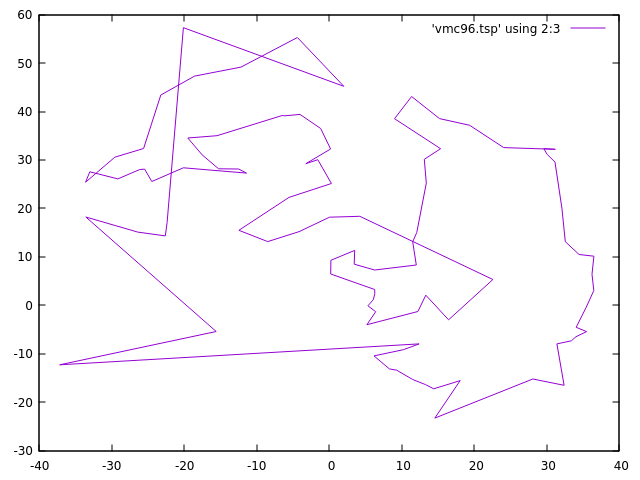
\includegraphics[width=\textwidth]{gr96_vmc.png}
\caption*{\small{Vecino más cercano}}
\end{subfigure}
\quad
\begin{subfigure}[b]{0.36\textwidth}
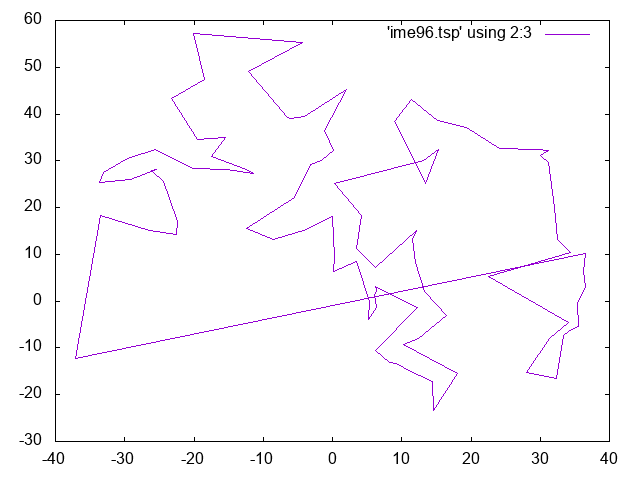
\includegraphics[width=\textwidth]{gr96_ime.png}
\caption*{\small{Inserción más económica}}
\end{subfigure}

\vspace{0.25cm}

\begin{subfigure}[b]{0.36\textwidth}
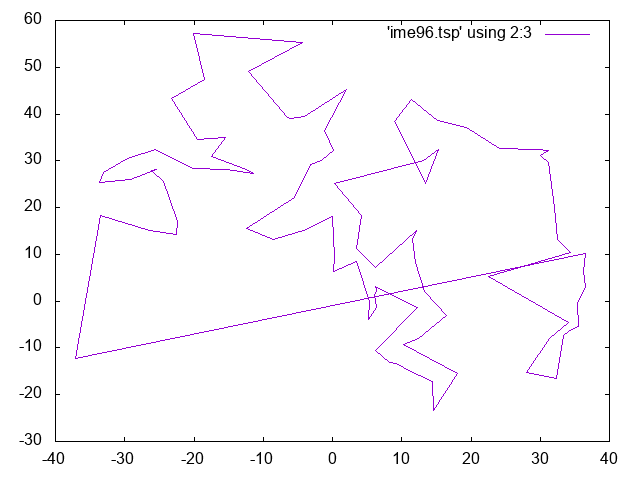
\includegraphics[width=\textwidth]{gr96_ime.png}
\caption*{\small{Derivado de Kruskal}}
\end{subfigure}
\quad
\begin{subfigure}[b]{0.36\textwidth}
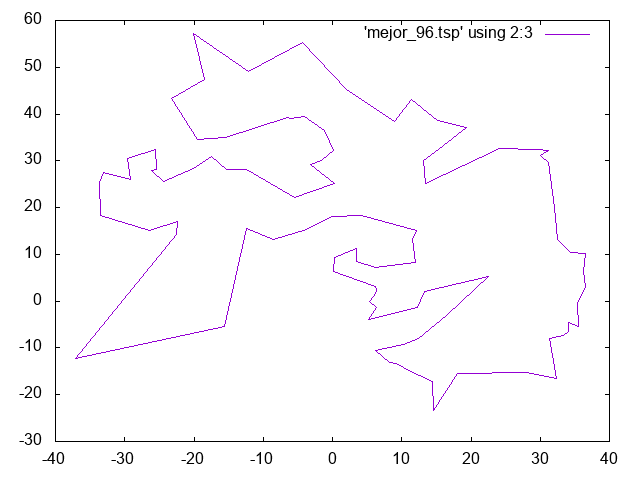
\includegraphics[width=\textwidth]{gr96_mejor.png}
\caption*{\small{Versión óptima}}
\end{subfigure}
\end{figure}

\end{frame}
%%%%%%%%%%%%%%%%%%
\begin{frame}[fragile]{\textit{a280.tsp}}
\begin{figure}[H]
\centering
\begin{subfigure}[b]{0.36\textwidth}
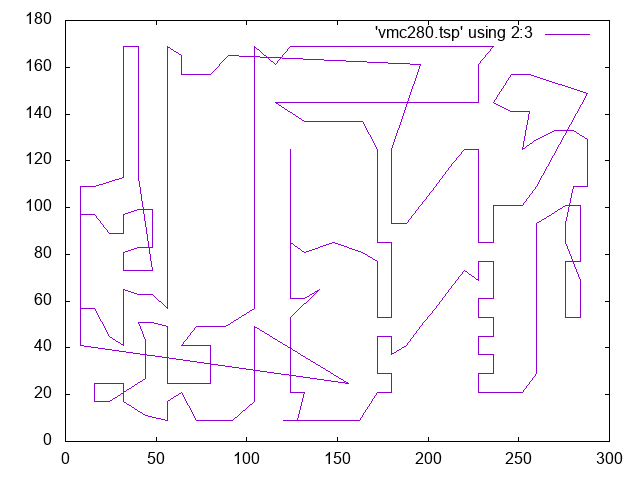
\includegraphics[width=\textwidth]{a280_vmc.png}
\caption*{\small{Vecino más cercano}}
\end{subfigure}
\quad
\begin{subfigure}[b]{0.36\textwidth}
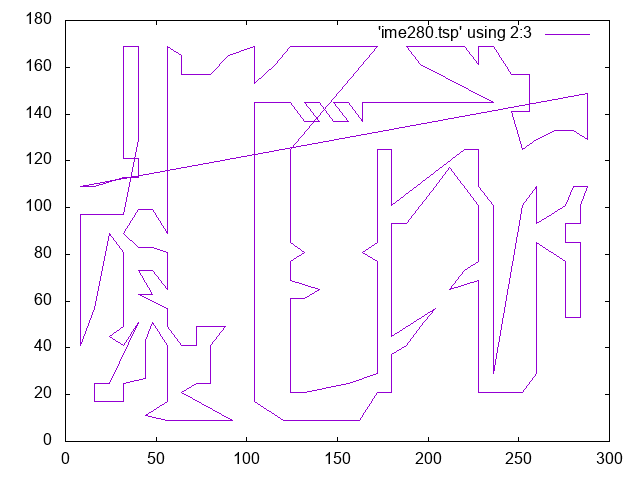
\includegraphics[width=\textwidth]{a280_ime.png}
\caption*{\small{Inserción más económica}}
\end{subfigure}

\vspace{0.25cm}

\begin{subfigure}[b]{0.36\textwidth}
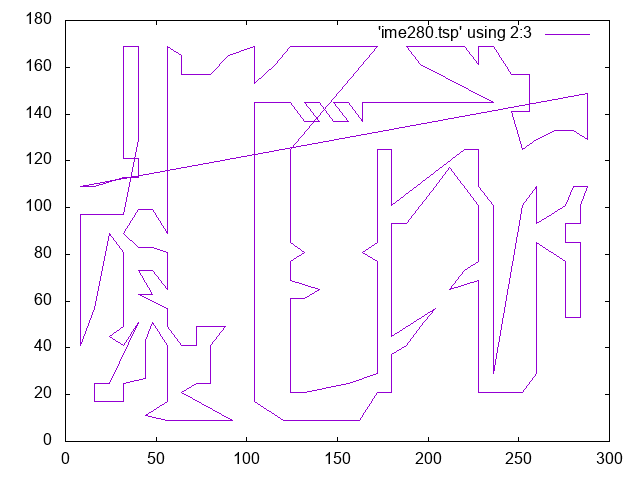
\includegraphics[width=\textwidth]{a280_ime.png}
\caption*{\small{Derivado de Kruskal}}
\end{subfigure}
\quad
\begin{subfigure}[b]{0.36\textwidth}
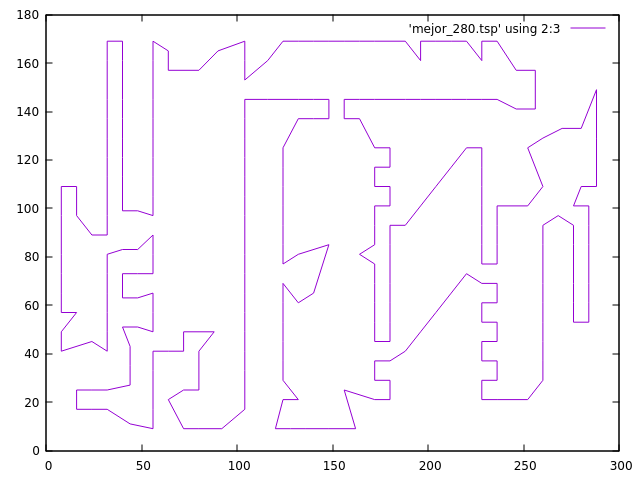
\includegraphics[width=\textwidth]{a280_mejor.png}
\caption*{\small{Versión óptima}}
\end{subfigure}
\end{figure}

\end{frame}

%%%%%%%%%%%%%%%%%%
\begin{frame}[fragile]{\textit{tsp225.tsp}}
\begin{figure}[H]
\centering
\begin{subfigure}[b]{0.36\textwidth}
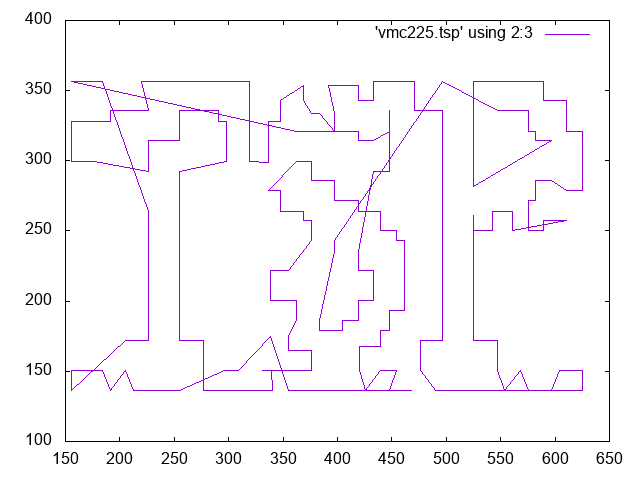
\includegraphics[width=\textwidth]{tsp225_vmc.png}
\caption*{\small{Vecino más cercano}}
\end{subfigure}
\quad
\begin{subfigure}[b]{0.36\textwidth}
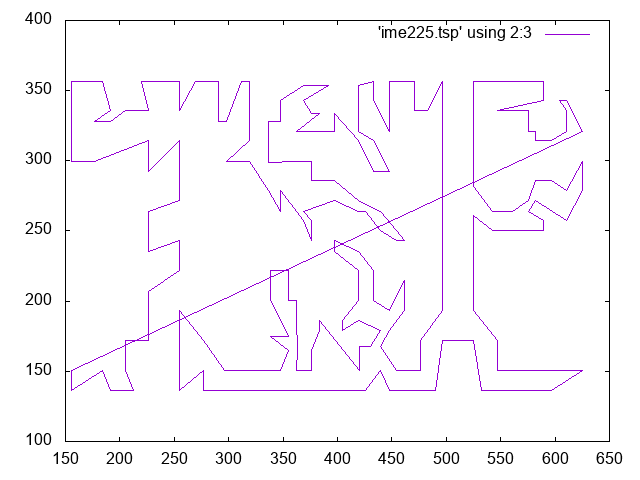
\includegraphics[width=\textwidth]{tsp225_ime.png}
\caption*{\small{Inserción más económica}}
\end{subfigure}

\vspace{0.25cm}

\begin{subfigure}[b]{0.36\textwidth}
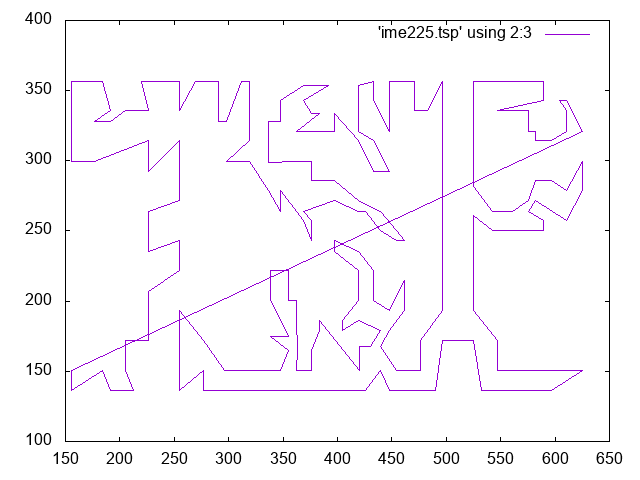
\includegraphics[width=\textwidth]{tsp225_ime.png}
\caption*{\small{Derivado de Kruskal}}
\end{subfigure}
\quad
\begin{subfigure}[b]{0.36\textwidth}
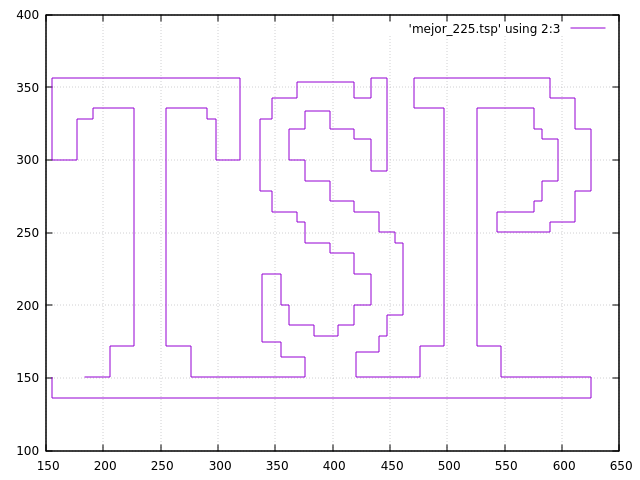
\includegraphics[width=\textwidth]{tsp225_mejor.png}
\caption*{\small{Versión óptima}}
\end{subfigure}
\end{figure}

\end{frame}


%%%%%%%%%%%%%%%%%%
\begin{frame}[fragile]{\textit{st70.tsp}}
\begin{figure}[H]
\centering
\begin{subfigure}[b]{0.36\textwidth}
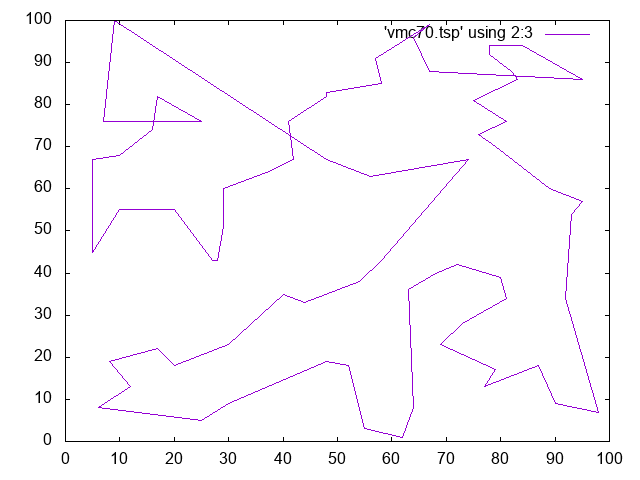
\includegraphics[width=\textwidth]{st70_vmc.png}
\caption*{\small{Vecino más cercano}}
\end{subfigure}
\quad
\begin{subfigure}[b]{0.36\textwidth}
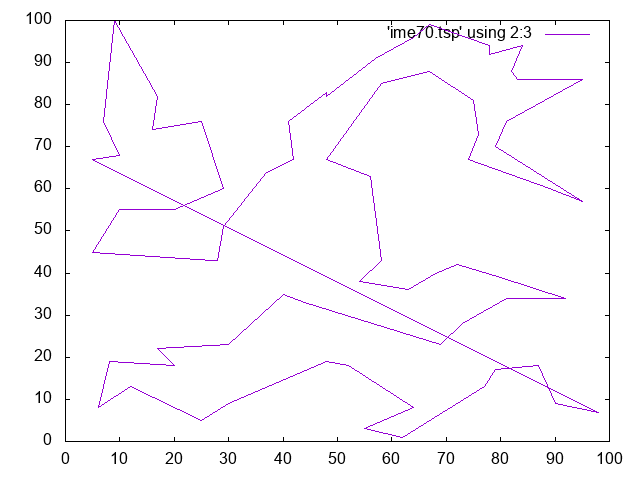
\includegraphics[width=\textwidth]{st70_ime.png}
\caption*{\small{Inserción más económica}}
\end{subfigure}

\vspace{0.25cm}

\begin{subfigure}[b]{0.36\textwidth}
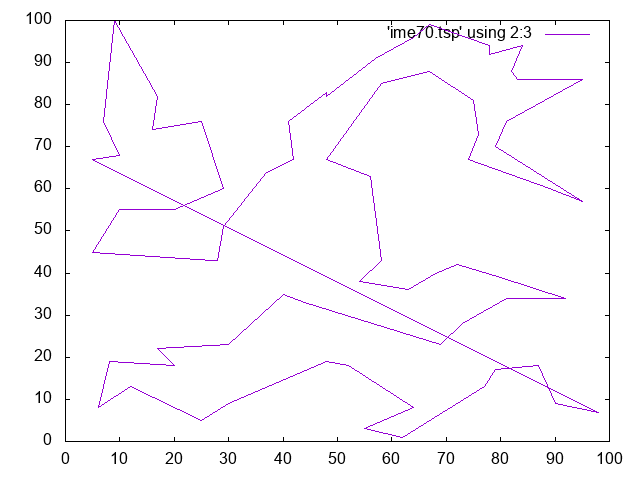
\includegraphics[width=\textwidth]{st70_ime.png}
\caption*{\small{Derivado de Kruskal}}
\end{subfigure}
\quad
\begin{subfigure}[b]{0.36\textwidth}
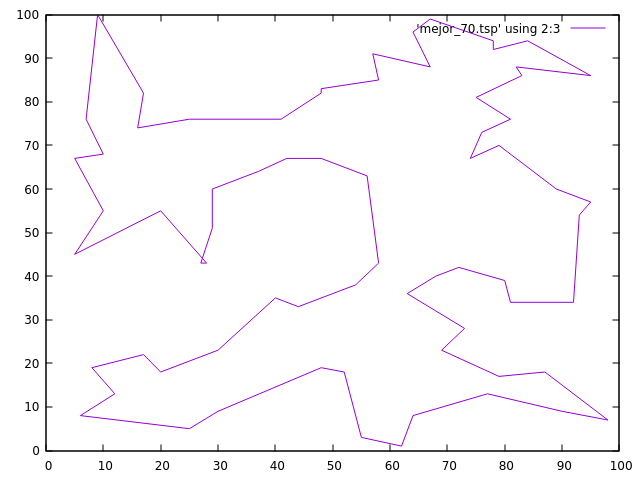
\includegraphics[width=\textwidth]{st70_mejor.png}
\caption*{\small{Versión óptima}}
\end{subfigure}
\end{figure}

\end{frame}	


\begin{frame}[fragile]{Resultados obtenidos}
\begin{figure}[H]
\centering

\adjustbox{max height=\dimexpr\textheight-5.5cm\relax,
           max width=\textwidth}{
\begin{tabular}{|c|c|c|c|c|}
\hline
 & \textit{gr96.tsp} & \textit{a280.tsp} & \textit{tsp225.tsp} & \textit{st70.tsp}\\
 \hline
 \small{\textbf{Vecino más cercano}} & 603.302 & 3094.28 & 4633.2 & 761.689 \\
 \hline
 \small{\textbf{Inserción más económica}} & 620.367 & 3192.42 & 4734.51 & 824.228 \\
 \hline
 \small{\textbf{Derivado de Kruskal}} & & & &\\
 \hline
 \small{\textbf{Solución óptima}} & 512.309 & 2586.77 & 3859 & 678.597 \\
 \hline
\end{tabular}
}
\end{figure}

\end{frame}	


\section*{Fin de la presentación}

\begin{frame}{Fin}
\begin{center}
\huge{Fin de la presentación}
\end{center}
\end{frame}


\end{document}


